\documentclass[12pt,a4paper]{article}
\usepackage[UTF8]{ctex}
\usepackage{amsmath, amssymb}
\usepackage{geometry}
\usepackage{booktabs}
\usepackage{graphicx}
\usepackage{float}
\geometry{left=2.5cm, right=2.5cm, top=2.5cm, bottom=2.5cm}
\title{\textbf{问题三 灵敏度分析报告}\\[4pt]
\large VLSI 布图规划设计 --- 判定强度参数灵敏度分析}
\author{2026 年第七届"华数杯"大学生数学建模竞赛 B 题}
\date{2026/08}
\begin{document}
\maketitle

\section{S1：判定种子数灵敏度}

可行性判定是启发式的，存在假阴性（搜索不足被判不可行）。判定种子数
$K$ 直接决定假阴性概率（$P \approx \prod P_s$）。扫描
$K = 1/3/5/7/10/15$（n100/n200），n300 扫描至 5/7/10
（seed15/20 因赛程时间未加密）。

\begin{figure}[H]
\centering
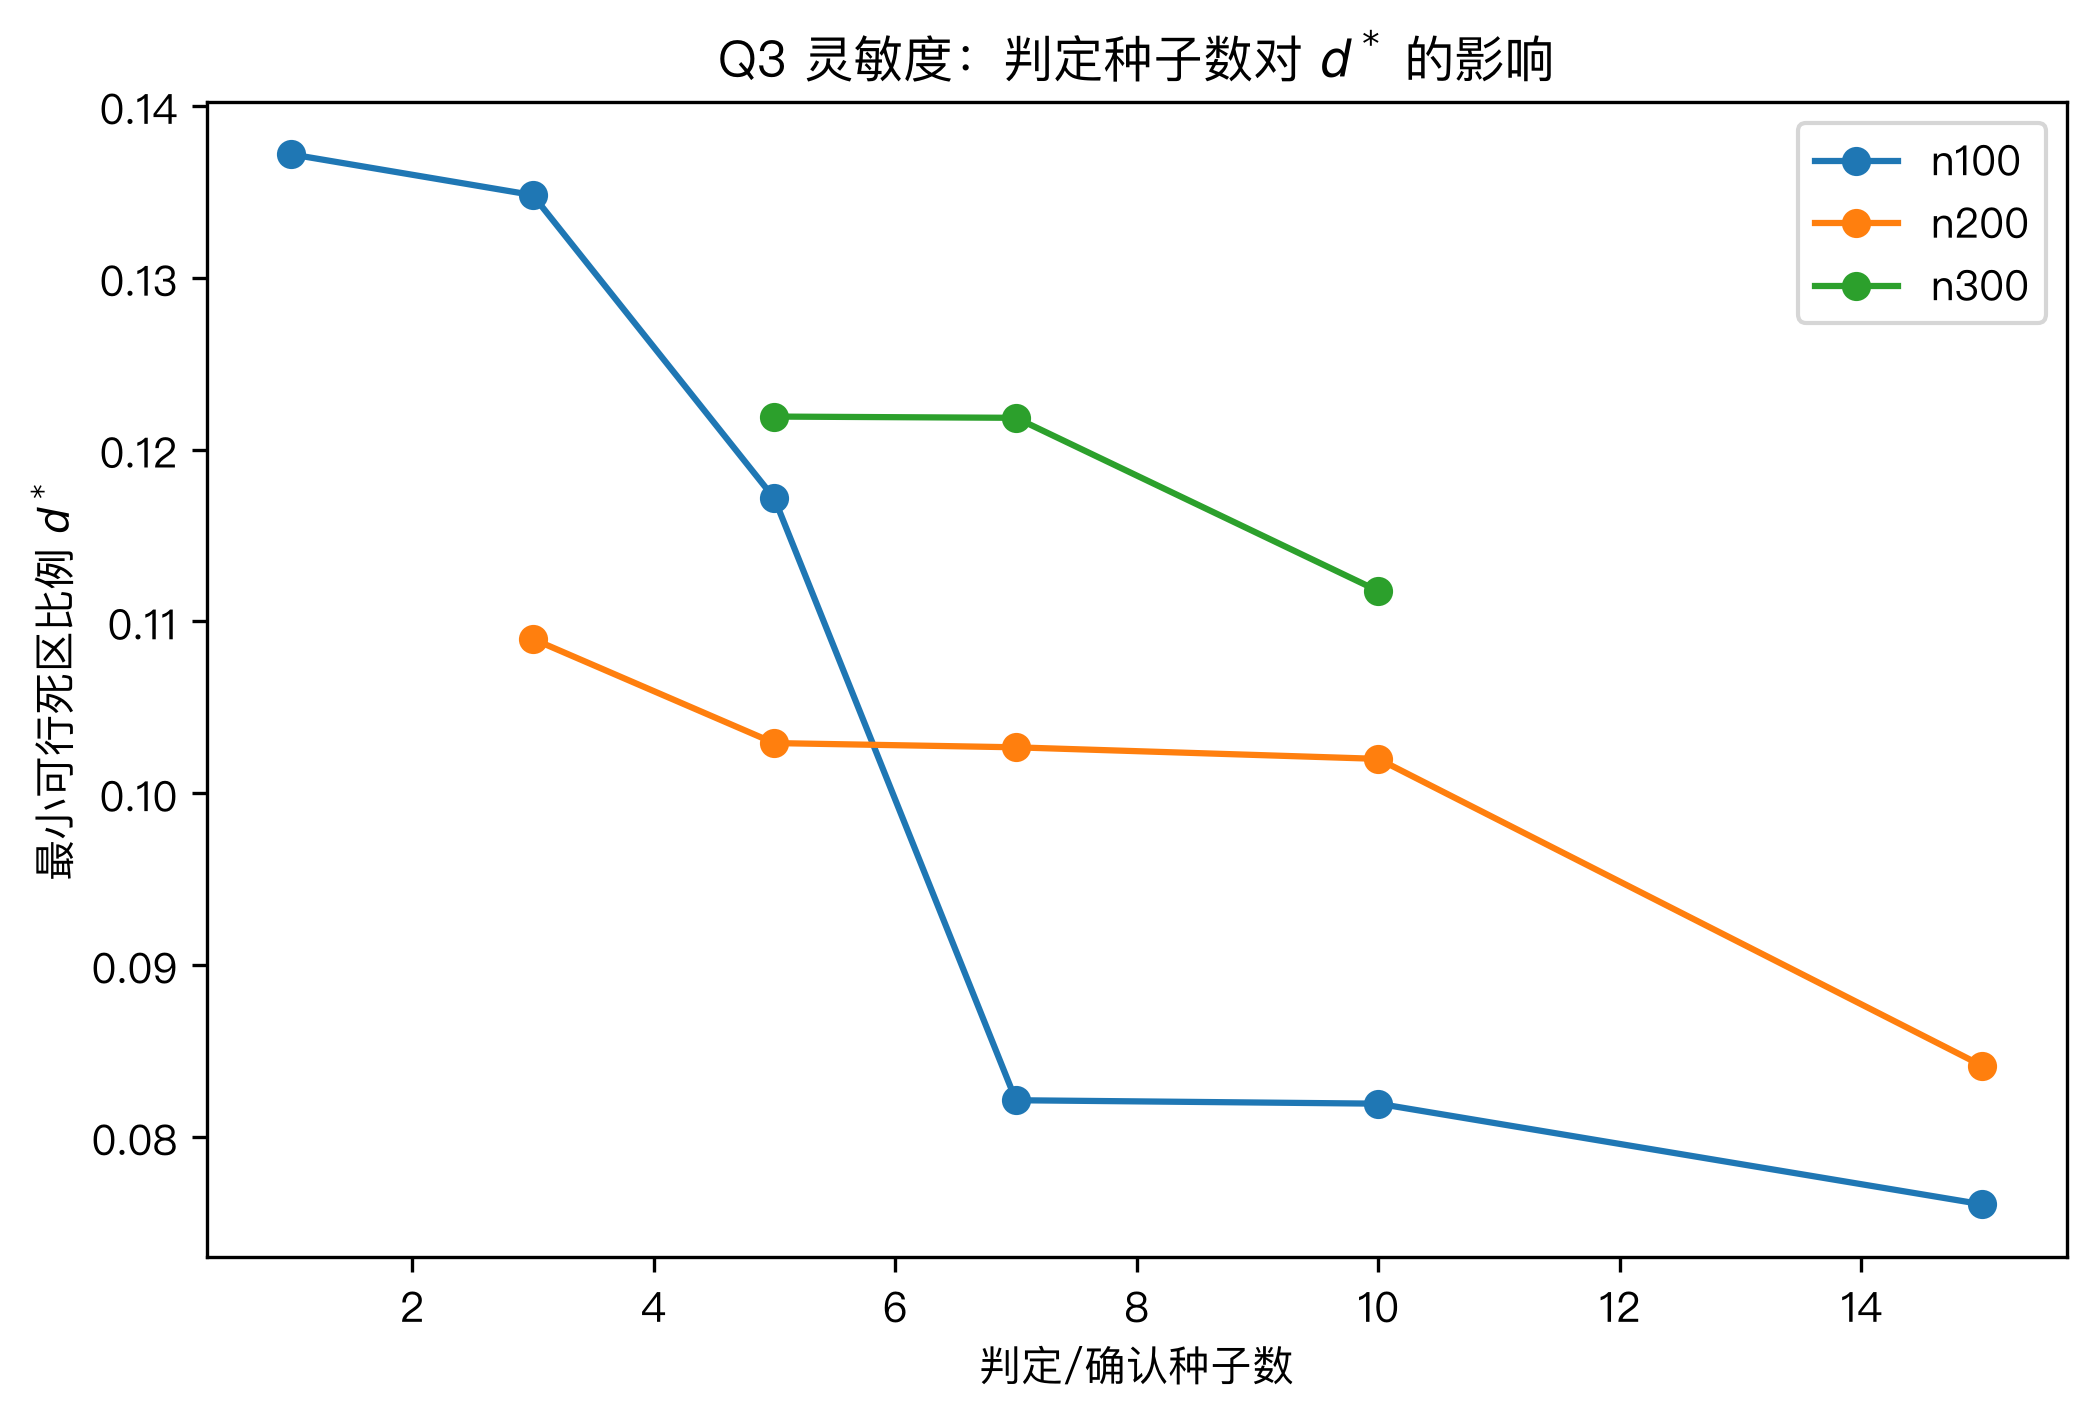
\includegraphics[width=0.82\textwidth]{../../图表/Q3/图/q3_seed_sensitivity.png}
\caption{$d^*$ 随判定种子数变化}
\end{figure}

  \begin{table}[H]
  \centering
  \caption{S1 数据（eps=1e-4）}\label{tab:q3s1}
  \begin{tabular}{llll}
  \toprule
  chip & seeds & d\_star & confirmed \\
  \midrule
  n100 & 1 & 0.137183 & True \\
  n100 & 3 & 0.134811 & False \\
  n100 & 5 & 0.117161 & True \\
  n100 & 7 & 0.082131 & True \\
  n100 & 10 & 0.081931 & True \\
  n100 & 15 & 0.076072 & True \\
  n200 & 3 & 0.108977 & True \\
  n200 & 5 & 0.102918 & True \\
  n200 & 7 & 0.102671 & True \\
  n200 & 10 & 0.101998 & False \\
  n200 & 15 & 0.084141 & True \\
  n300 & 5 & 0.121921 & True \\
  n300 & 7 & 0.121848 & True \\
  n300 & 10 & 0.111773 & True \\
  \bottomrule
  \end{tabular}
  \end{table}

\textbf{结论}：$d^*$ 随种子数\textbf{单调下降}——n100 从 1 种子的
0.137183 降至 15 种子的 0.076072（改善 45\%），n200 从 3 种子的
0.108977 降至 15 种子的 0.084141（改善 23\%），n300 从 5 种子的
0.121921 降至 10 种子的 0.111773（改善 8\%）。种子数 3 时 n100
判定不可靠（未确认），5 及以上稳定。\emph{论文表述必须注明
"搜索强度相关"}：$d^*$ 是在当前判定强度下验证过的最小可行死区比例；
定稿协议为 n100/n200 判定 15、n300 判定 10（n300 的 15/20 因赛程
未扫描，可按需加密）。

\section{S2：二分终止精度灵敏度}

二分终止条件 $hi - lo < \varepsilon$，扫描
$\varepsilon = 10^{-3}/10^{-4}/10^{-5}$（n100，seeds=3）。

\begin{figure}[H]
\centering
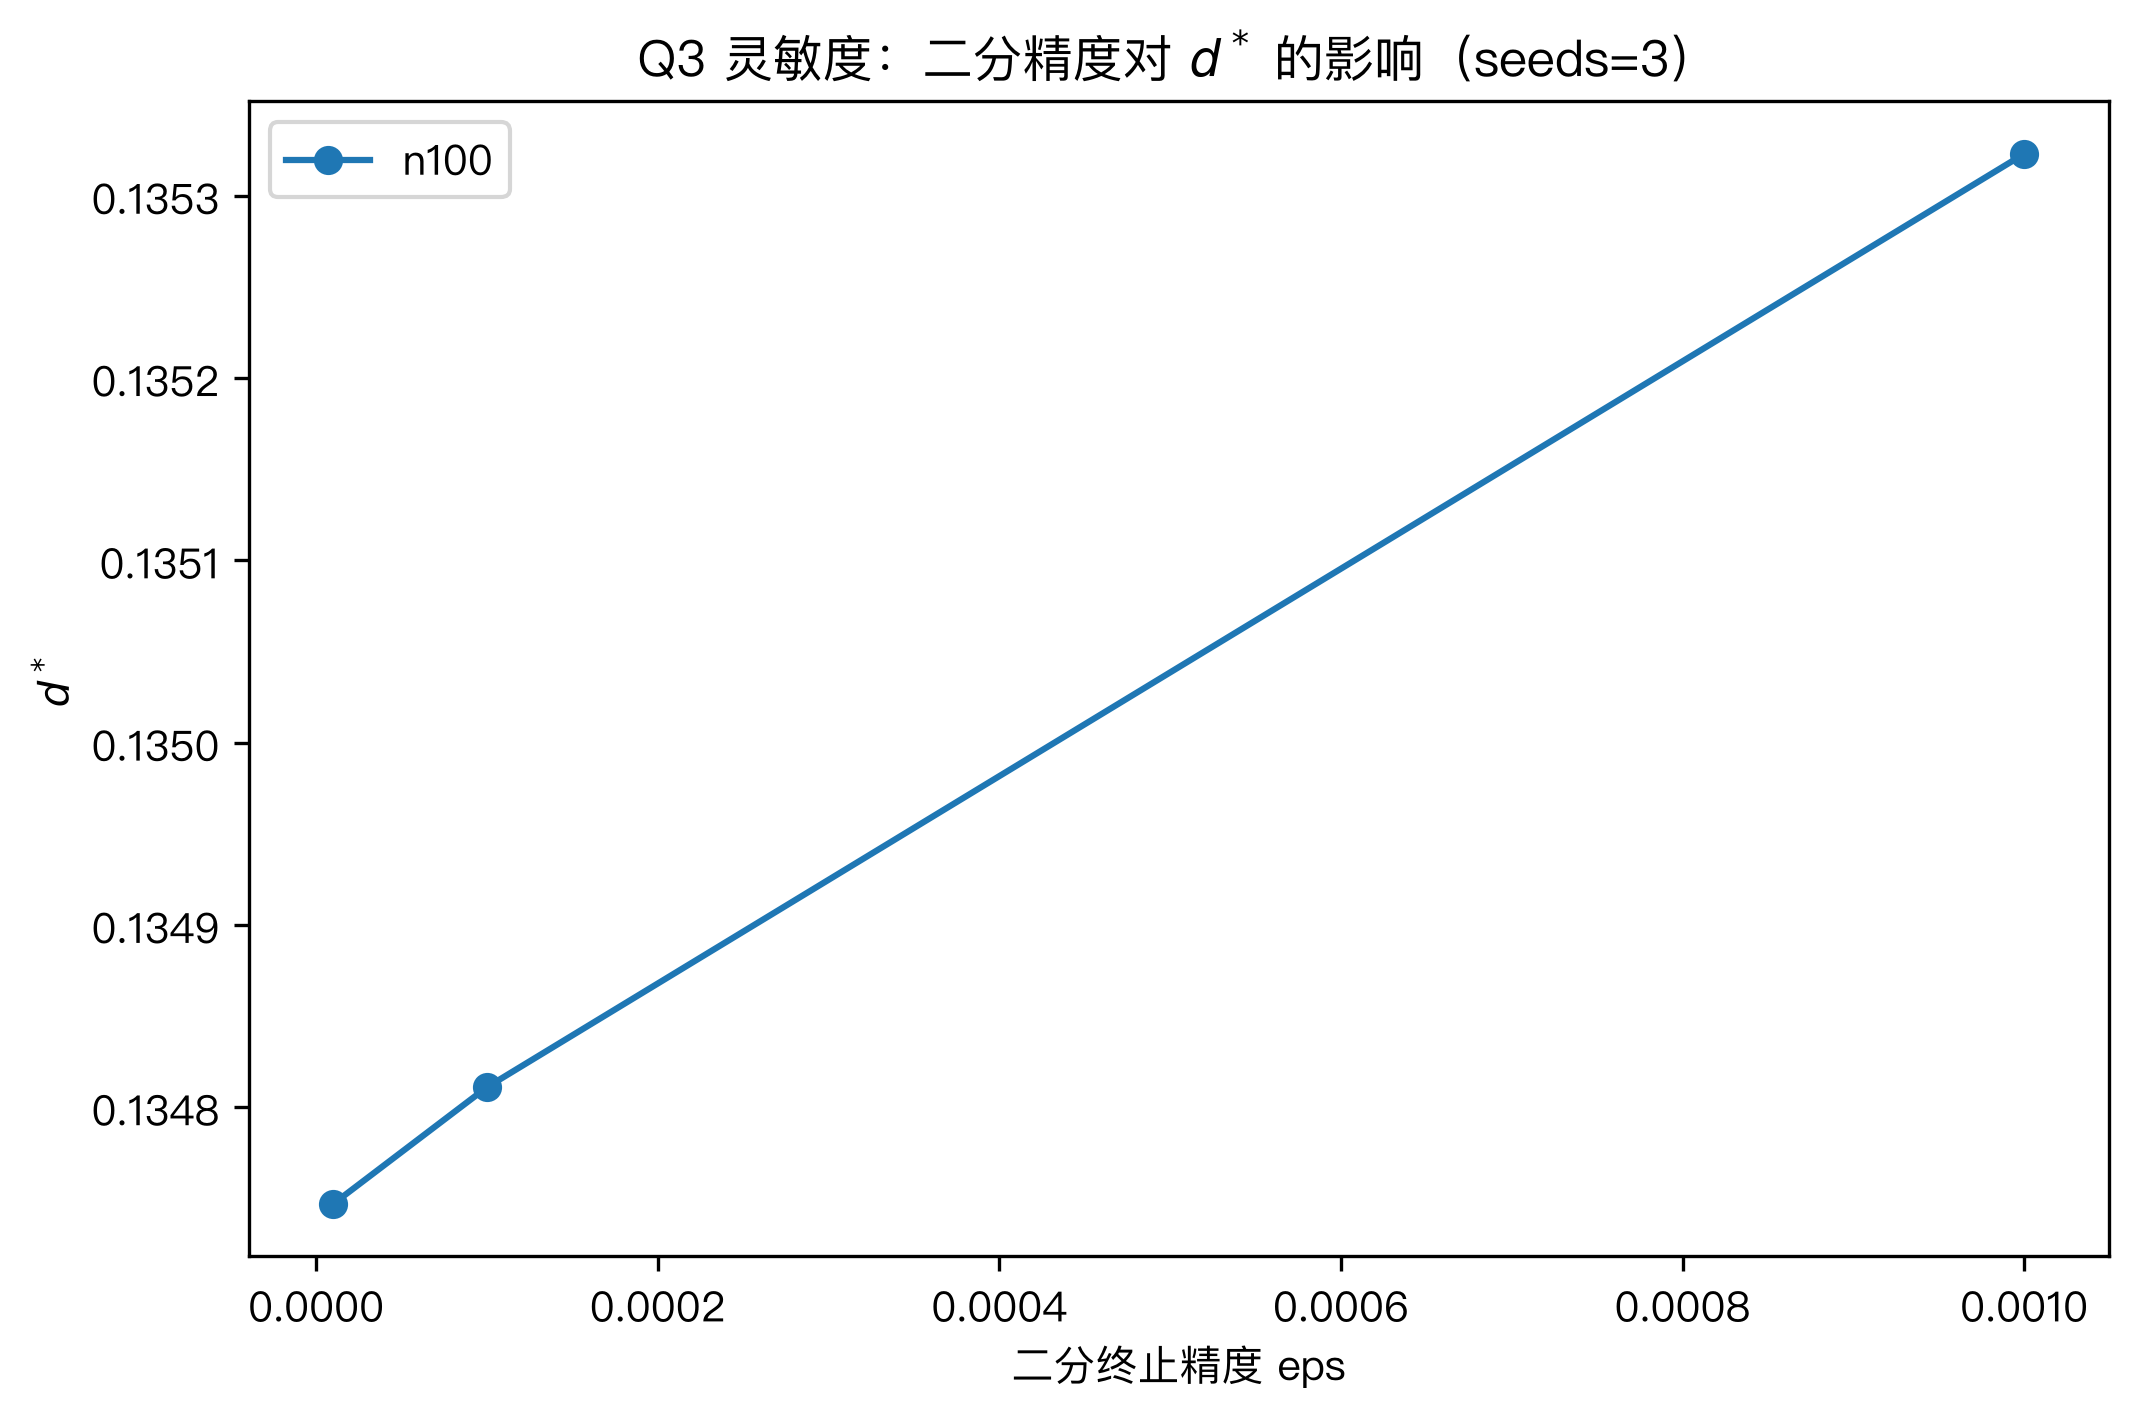
\includegraphics[width=0.82\textwidth]{../../图表/Q3/图/q3_eps_sensitivity.png}
\caption{$d^*$ 随二分精度变化}
\end{figure}

  \begin{table}[H]
  \centering
  \caption{S2 数据}\label{tab:q3s2}
  \begin{tabular}{lll}
  \toprule
  chip & eps & d\_star \\
  \midrule
  n100 & 1e-05 & 0.134747 \\
  n100 & 0.0001 & 0.134811 \\
  n100 & 0.001 & 0.135323 \\
  \bottomrule
  \end{tabular}
  \end{table}

\textbf{结论}：$\varepsilon$ 从 $10^{-3}$ 收紧到 $10^{-5}$，
$d^*$ 仅变化 0.4\%（0.135323 $\to$ 0.134747）——二分精度对结果
\textbf{不敏感}，$10^{-4}$ 是成本与精度的合理平衡点（约 11 次判定）。

\section{S3：判定/确认种子解耦}

二分判定（judge）与最终双向确认（confirm）使用不同的种子数，
扫描判定 3/5 $\times$ 确认 7/10。

\begin{figure}[H]
\centering
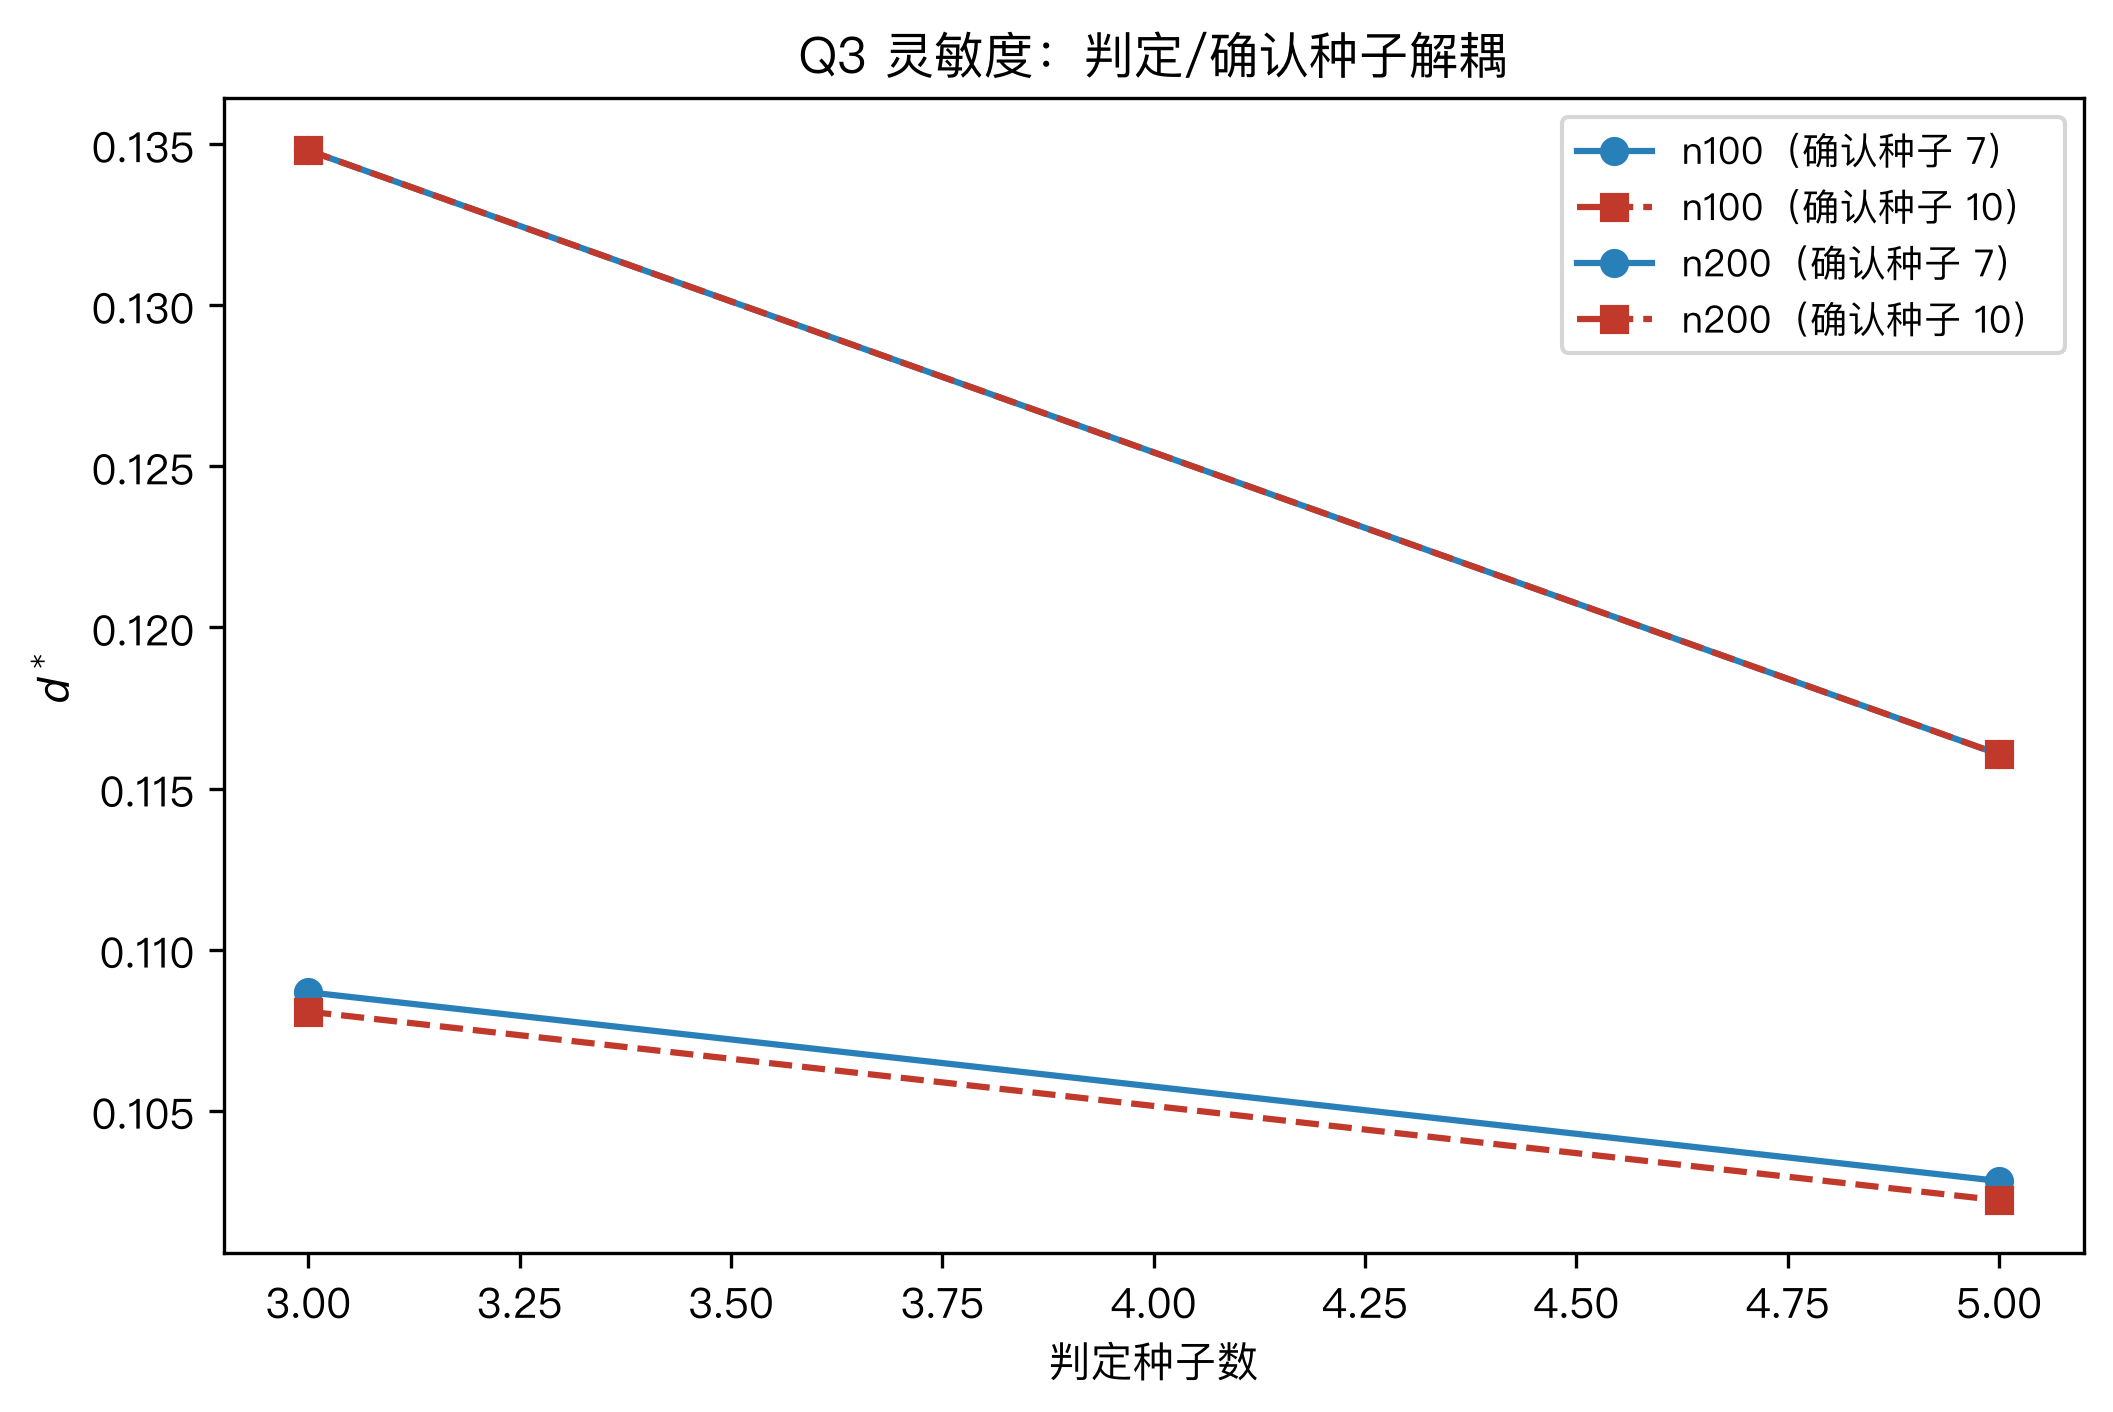
\includegraphics[width=0.82\textwidth]{../../图表/Q3/图/q3_sep_judge_confirm.png}
\caption{判定/确认种子解耦对 $d^*$ 的影响}
\end{figure}

  \begin{table}[H]
  \centering
  \caption{S3 数据}\label{tab:q3s3}
  \begin{tabular}{lllll}
  \toprule
  chip & judge\_seeds & confirm\_seeds & d\_star & confirmed \\
  \midrule
  n100 & 3 & 7 & 0.134811 & False \\
  n100 & 3 & 10 & 0.134811 & False \\
  n100 & 5 & 7 & 0.116061 & False \\
  n100 & 5 & 10 & 0.116061 & False \\
  n200 & 3 & 7 & 0.108677 & True \\
  n200 & 3 & 10 & 0.108077 & False \\
  n200 & 5 & 7 & 0.102818 & True \\
  n200 & 5 & 10 & 0.102218 & False \\
  n300\_n300 & 5 & 10 & 0.121021 & True \\
  \bottomrule
  \end{tabular}
  \end{table}

\textbf{结论}：\textbf{判定种子决定 $d^*$ 位置}（3 $\to$ 5 时
$d^*$ 从 0.134811 降至 0.116061），确认种子决定"确认"成败
（判定 5 + 确认 7 未通过，需更小的 $d^*$ 才能通过）——两者解耦验证了
"判定强度 $\rightarrow$ 假阴性率 $\rightarrow$ $d^*$ 精度"的因果链，
支持交付采用高判定/确认种子协议。

\end{document}
